\documentclass[14pt]{extreport}
\usepackage[T1]{fontenc}
\usepackage[left=1in, right=1in, top=1in, bottom=1in]{geometry}
\usepackage{amsmath, amssymb, amsthm}
\usepackage{enumitem}
\usepackage{mathtools}
\usepackage{cancel}


\usepackage{bm}
% colored links
\usepackage{hyperref}
\hypersetup{
    colorlinks=true,
    linkcolor=blue,
    filecolor=magenta,      
    urlcolor=black!20!BurntOrange,
    }

% Inputting Python code
\usepackage[dvipsnames]{xcolor}
\definecolor{textblue}{rgb}{.2,.2,.7}
\definecolor{textred}{rgb}{0.54,0,0}
\definecolor{textgreen}{rgb}{0,0.43,0}
\usepackage{upquote}
\usepackage{listings}
\lstset{
    language=Python, 
    tabsize=4,
    basicstyle={\ttfamily},
    keywordstyle=\color{textblue},
    commentstyle=\color{textgreen},
    stringstyle=\color{textred},
    frame=none,
    columns=fullflexible,
    keepspaces=true,
    showstringspaces=false,
    xleftmargin=-15mm, % manual adjustment, figure out permanent solution
}

% Drawing figures
\usepackage{tikz}
\usetikzlibrary{matrix, positioning}
\usetikzlibrary{calc, shapes.symbols}
\usepackage{pgfplots}
\pgfplotsset{compat=newest}

% Colored Boxes
\usepackage{tcolorbox}
\tcbuselibrary{skins,hooks}
\usetikzlibrary{shadows}
\usepackage{lipsum}

%Easy Numbering in case we add or remove questions
\newcounter{counter}
\newcommand{\Exercise}{Exercise \stepcounter{counter}\thecounter}

%Images
\usepackage{graphicx}
    \usepackage{subcaption}
    \usepackage{float}

%Formatting and Spacing
\setitemize[1]{noitemsep, parsep = 5pt, topsep = 5pt}
\setenumerate[1]{label = (\alph*), parsep = 1pt, topsep = 5pt}
\setlength\parindent{0pt}
\linespread{1.1}

%Cases Environment
\newlist{Cases}{enumerate}{3}
\setlist[Cases]{leftmargin = .25in, label = {Case \arabic*.}, topsep = 0.01in, itemsep = 0.04in, itemindent = .5in, parsep = 0in}

%Stats
\newcommand{\Cov}{\text{Cov}}
\newcommand{\trace}{\text{trace}}
\newcommand{\Normal}{\text{Normal}}
\newcommand{\Var}[1]{\operatorname{Var}\left(#1\right)}
\newcommand{\E}[2][]{\operatorname{E}_{#1}\left[#2\right]}
\DeclareMathOperator*{\oldPr}{Pr}
\renewcommand{\Pr}[2][]{\operatorname{Pr}_{#1}\left(#2\right)}

%Custom Title Fields
\newcommand{\lectTitle}{Exam 2 Review}
\newcommand{\lectTime}{March 7, 2022}
\newcommand{\lectClass}{Advanced Algorithms}
\newcommand{\lectClassInstructor}{Dana Randall}
\newcommand{\lectSection}{Spring 2024}
\newcommand{\lectAuthorName}{Sarthak Mohanty}


\title{
    \vspace{1.75in}
    \textbf{\lectClass:\\ \lectTitle}\\
    \vspace{0.1in}\large{\textit{\lectClassInstructor\ \lectSection}}
    \vspace{2in}
    \author{\textbf{Sarthak Mohanty}}
    \date{}
}

\begin{document}

\maketitle
\pagebreak

\subsection*{\Exercise}
Short-answer questions. No justification required.
\begin{enumerate}
    \item Consider Fortune’s algorithm to compute the Voronoi diagram of n sites in
    the plane. What is the maximum number of arcs that any one site can contribute to the
    beach line?
    \item Which of the following assertions about the Delaunay triangulation (DT) of
    a set $P$ of $n$ points in the plane are always true? Select all that apply.
    \begin{enumerate}[label=\roman*.]
    \small
        \item The closest pair of points are connected by an edge in the DT.
        \item The farthest pair of points cannot be connected by an edge in the DT.
        \item Among all triangulations of P, the DT maximizes the minimum angle.
        \item Among all triangulations of P, the DT minimizes the maximum angle.
        \item Among all triangulations of P, the DT minimizes the total sum of edge lengths
    \end{enumerate}
    \item Recall the \textsf{Max3SAT} problem. The input is a Boolean formula in conjunctive normal form and you wish to output an assignment of the variables that satisfy the maximum number of clauses. True or false: there exists an $\epsilon$-approximation for the \textsf{Max3SAT} problem for any $\epsilon > 0$.
    \item True or false: there exists a 2-approximation for the TSP problem.
\end{enumerate}

\subsection*{\Exercise}
    \textit{(Erickson)} Suppose you are a TA for a computational geometry class. You’re allowing the students to use their own favorite programming language and programming environment, which means you can’t compile the code yourself. Thus, instead of submitting the code itself, you asked your students to submit several Voronoi diagrams computed by their code
    
    \vspace{3mm}
    After the submission deadline, you realize that you forgot to ask the students to submit the sites that defined each of their Voronoi diagrams! In frustration, you decide to give your students full credit if every diagram they submit is the Voronoi diagram of some point set. But how do you tell?\footnote{I had a similar issue as a TA for \href{https://github.com/sar-mo/CS2051-HonorsDiscreteMath/blob/main/sp23/hw-supplements/hw3-supp/images/colored_map2.pdf}{2051}.}

    \vspace{3mm}
    Describe and analyze an algorithm to determine, given a planar straight-line graph G, whether $G$ is a Voronoi diagram. Your algorithm should either return a finite point set $P$ such that $G$ is the Voronoi diagram of P, or report correctly that no such point set exists. [\textit{Hint:} Consider the case of four sites.]

\subsection*{\Exercise}
    \textit{(Mount)} In class we proved that the Delaunay triangulation of a set of sites in the plane maximizes the
    minimum angle. (It is the max-min angle triangulation.) Unfortunately, it is not the best triangulation
    for the following two criteria.
    \begin{enumerate}
        \item Give an example of a set of point sites in the plane such that the Delaunay triangulation of this set does not minimize the sum of edge lengths, among all possible triangulations. In other words, the Delaunay triangulation is not the minimum-weight triangulation.
        \item Give an example of a set of point sites in the plane such that the Delaunay triangulation of this point set does not minimize the maximum angle, among all possible triangulations. In other words, the Delaunay triangulation is not the min-max angle triangulation.
    \end{enumerate}
    In each case briefly explain your construction. Your example should be in general position (e.g., no
    four sites should be cocircular).
    
    \vspace{2mm}
    \textit{Hint:} In both cases, it is possible build a counterexample consisting of just four points that are nearly co-circular. It suffices to present a single, specific example.

\subsection*{\Exercise\footnote{From Princeton COS 226 Final Exam.}}
Suppose you want to compute a Voronoi data structure for a set of pixels drawn from an \( R \)-by-\( R \) grid. Devise an efficient scheme to support the following three operations.

\begin{itemize}
  \item \texttt{create(R)}: create an empty data structure to handle an \( R \)-by-\( R \) grid.
  \item \texttt{insert(i,j)}: insert the pixel \( (i,j) \) into the data structure, where \( i \) and \( j \) are integers between \( 0 \) and \( R-1 \).
  \item \texttt{find(x,y)}: return the inserted pixel which is closest to \( (x,y) \) in Euclidean distance, where \( x \) and \( y \) are integers between \( 0 \) and \( R-1 \).
\end{itemize}

The \texttt{create} and \texttt{insert} operation should take \( \mathcal{O}(R^2) \) time; the \texttt{find} operation should take \( \mathcal{O}(1) \) time. For partial credit, give an algorithm that takes \( \mathcal{O}(NR^2) \) time for \texttt{insert}, where \( N \) is the number of points already inserted into the data structure. (\textit{Hint:} think simple.)

\begin{enumerate}[label=(\alph*)]
  \item Describe how to implement \texttt{create(R)}. Indicate what is being stored.
  \item Describe how to implement \texttt{find(i,j)}.
  \item Describe how to implement \texttt{insert(i,j)}.
\end{enumerate}

\subsection*{\Exercise}
    Assess the validity of the following claim: ``If there exists an $\epsilon$ such that \textsf{MaxClique} is $\epsilon$-approximable, then \textsf{MaxClique} is also $\frac{\epsilon}{4}$-approximable." If true, then give a $\frac{\epsilon}{4}$-appoximation for \textsf{MaxClique}. If false, provide a counterexample or reasoning to demonstrate why the claim does not hold.

% \subsection*{Solution}
%     The first thing to note is that any empty circle of maximal radius will have its center on the Voronoi diagram. If a circle is of maximal radius, it must have on its boundary at least two of the $n$ sites, otherwise we could make it bigger. These two sites are then equidistant from the circle's centers, and the Voronoi diagram contains all points equidistant from at least two sites. 

%     \vspace{3mm}
%     Suppose you start with a circle whose center is inside the convex hull on some edge of the Voronoi diagram, equidistant from two sites.  By sliding the center of the circle along the Voronoi edge, you can make the circle bigger. You can do this until one of two things occurs. First, if you reach a vertex of the Voronoi diagram, the center of the circle is now equidistant from at least three sites, and the circle cannot be made any bigger since three points determine a unique circle. Secondly, you could slide the center until it is about to leave the convex hull. At that point the circle can't be made any bigger without moving the center outside the convex hull something we want to avoid. We note that this only occurs for non-infinite edges, as any circle centered at the intersection of an infinite edge with the convex hull could be made larger by moving the center of this circle inward. 

%     \vspace{3mm}
%     So, we've characterized all the local maxima for empty circles: their centers are either at vertices of the Voronoi diagram inside the convex hull, or at the intersections of finite edges of the Voronoi diagram and the convex hull.  We can now find the largest of all these with the following algorithm:
%     \begin{enumerate}
%         \item Find the Voronoi diagram of the sites. 
%         \item For each vertex of the Voronoi diagram, check whether it is inside the convex hull. 
%         \begin{enumerate}
%             \item If it is, find the distance to the closest sites, which is the size of the largest empty circle centered at the vertex.
%             \item If it is not, consider each non-infinite edge leaving the vertex, find where it intersects the convex hull, and calculate the radius of the largest empty circle centered at that intersection point
%         \end{enumerate}
%         \item Return the maximum
%     \end{enumerate}
%     By our arguments above, this algorithm will correctly find the largest empty circle because it considers all possible local maxima, and the largest empty circle must be a local maxima. Step 1 takes $\mathcal{O}(n \log n)$ time. Step 2 (a) takes constant time, and step 2 (b) takes amortized constant time: you can find which edges of the convex hull each edge of the Voronoi region cross in constant time, and even if one vertex has a linear number of edges the total number of edges considered across all iterations is $\mathcal{O}(n)$, which amortizes to constant edges per iteration. Determining in Step 2 which vertices are inside the convex hull across all iterations also takes $\mathcal{O}(n)$ time: for each vertex, you can check whether it is in the convex hull of its neighboring sites in time $\mathcal{O}($number of neighborings sites$)$. This is equal to the number of edges incident to the vertex, and summing across all vertices, this totals twice the number of edges, which is linear.  So step 2 take $\mathcal{O}(n)$ time total, and thus this algorithm runs in time $\mathcal{O}(n \log n)$. 

\subsection*{\Exercise}
    Prove that Chebyshev's inequality is tight: in other words, find a probability distribution for $X$ and a value $a$ such that
    \begin{equation*}
        \Pr{|X - \E{X}| \geq a} = \frac{\Var{X}}{a^2}.
    \end{equation*}
    \textit{Hint:} This random variable will take only three values.

\subsection*{\Exercise}
    As in the homework, consider the general problem where we have $m$ machines $M_1 \ldots M_m$ and a set of $n$ jobs. Each job $j$ has a processing time $t_j$. We seek to assign each job to one of the machines so that the loads placed on all machines are as "balanced" as possible. That is, if $A(i)$ are the set of jobs assigned to machine $M_i$ , then the load for machine $M_i$ is total time required.  \[ T_i = \sum_{j \in A(i)} t_j\] We want to minimize the $makespan$ $T = \max_i T_i$.
    \begin{enumerate}
        \item Describe a set of jobs such that the makespan of the greedy assignment is exactly $(2 - 1/m)$ times the makespan of the optimal assignment, where $m$ is the number of machines.
        \item  Describe an efficient algorithm to solve the minimum makespan scheduling
        problem exactly if every processing time $T_{i}$ is a power of two.
    \end{enumerate}

\subsection*{\Exercise}
    Run the Graham scan algorithm (as described in the lecture notes) to compute the convex hull of points below, starting from A. Give the points that appear on the trial hull (after each iteration) in the order that they appear.

    \begin{center}
    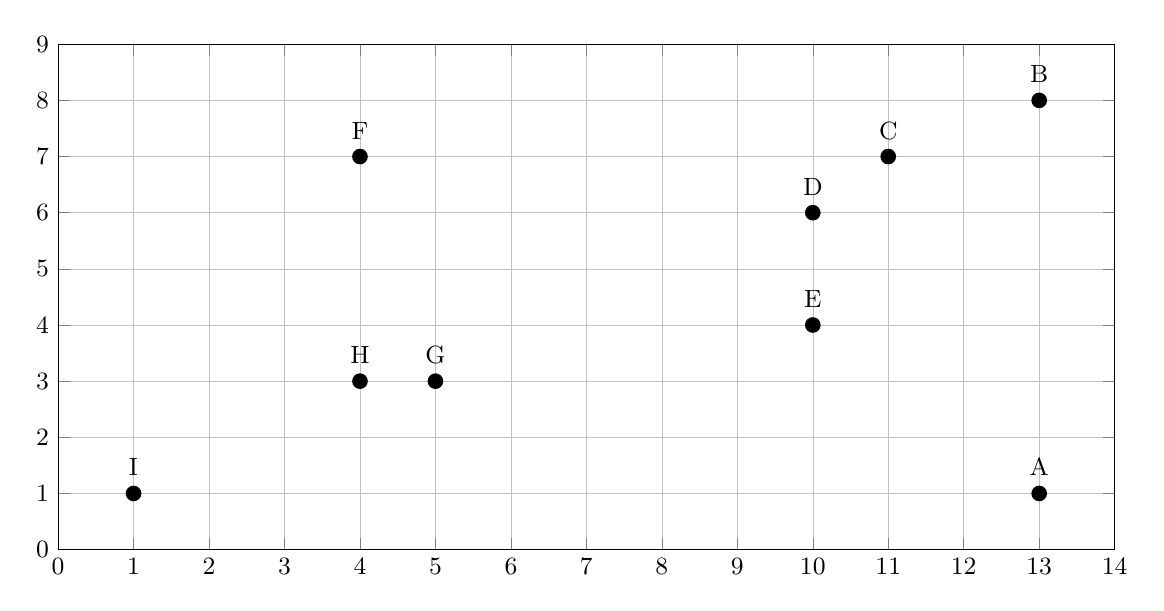
\begin{tikzpicture}[point/.style={circle,fill,inner sep=2pt}]
    \small
    \begin{axis}[
      xlabel={}, ylabel={},
      xmin=0, xmax=14,
      ymin=0, ymax=9,
      xtick={0,1,...,14},
      ytick={0,1,...,9},
      grid=both,
      major grid style={line width=.2pt,draw=gray!50},
      % enlargelimits={abs=0.5},
      % point meta=explicit symbolic,
        width=15cm, height=8cm % Adjust the size here to make the plot wider
    ]]
    
    % Points
    \node[label={90:{A}},point] at (axis cs:13,1) {};
    \node[label={90:{B}},point] at (axis cs:13,8) {};
    \node[label={90:{C}},point] at (axis cs:11,7) {};
    \node[label={90:{D}},point] at (axis cs:10,6) {};
    \node[label={90:{E}},point] at (axis cs:10,4) {};
    \node[label={90:{F}},point] at (axis cs:4,7) {};
    \node[label={90:{G}},point] at (axis cs:5,3) {};
    \node[label={90:{H}},point] at (axis cs:4,3) {};
    \node[label={90:{I}},point] at (axis cs:1,1) {};
    \end{axis}
    \end{tikzpicture}
    
        
    \end{center}

\subsection*{\Exercise}
    Again consider the following heuristic for constructing a vertex cover of a connected graph $G$: return the set of non-leaf nodes in any depth-first spanning tree of $G$. We know (from the homework) this algorithm is a 2-approximation to the minimum vertex cover. Describe an infinite family of graphs for which this heuristic returns a vertex cover of size $2 \cdot OPT$.

\subsection*{\Exercise}
    It is a fact that we still have no closed-form expression for the tail of the Normal distribution, which must be computed by numerically evaluating the integral. Let \(X \sim \mathcal{N}(0,1)\). Your goal is to produce upper bounds on \(P(X \geq a)\), where \(a > 0\).
    \begin{enumerate}
        \item Use Markov's inequality to bound \(\Pr{X \geq a}\). Note: This is not as trivial as it might seem because \(X\) is not non-negative. It will help to observe that:
        \[
        \Pr{X \geq a} = \Pr{X \geq a \mid X > 0} \cdot \Pr{X > 0}.
        \]
        Now define the non-negative r.v.\ \( Y = [X \mid X > 0] \) and note that \(\Pr{X \geq a \mid X > 0} = \Pr{Y \geq a}\).
        \item Use Chebyshev’s inequality to bound \(\Pr{X \geq a}\).
        \item \textit{(Optional)} Derive the Chernoff bound for \(\Pr{X \geq a}\).
    \end{enumerate}

\subsection*{\Exercise}
    Previously in this class, we discussed the \textbf{coupon collector} problem (do you remember when?) As a reminder: there are \( n \) distinct types of coupons you would like to collect. Each day you are sent a random coupon from among the \( n \) types. Let \( X \) denote the number of days needed to collect all \( n \) distinct coupons, given that coupons are chosen randomly with replacement. The following (famous) identity\footnote{known as the \href{https://en.wikipedia.org/wiki/Basel_problem}{Basel problem}.} is useful in answering some of the questions below:
    \[ \sum_{i=1}^{n} \frac{1}{i^2} = \frac{\pi^2}{6}. \]
    \begin{enumerate}
        \item What is \( \E{X}? \)\footnote{Of course we already discussed this in class, but good to practice!} What does this approach for high \( n \)? Write your answer using \( \mathcal{O}(\cdot) \).
        \item Derive \( \Var{X} \). What does this approach for high \( n \)? Write your answer using \( \mathcal{O}(\cdot) \).
        \item Derive an asymptotic upper bound on \( \Pr{X \geq 2n \ln(n)} \) for large \( n \) using Markov’s inequality.
        \item Derive an asymptotic upper bound on \( \Pr{X \geq 2n \ln(n)} \) for large \( n \) using Chebyshev’s inequality. Express your answer using \( \mathcal{O}(\cdot) \).
    \end{enumerate}
    Note: For \( \E{X} \) in (c) and (d), use the asymptotic mean from part (a).

\subsection*{\Exercise}
    \textit{(Erickson)}\ Recall that a family \(\mathcal{H}\) of hash functions is \textit{universal} if, for all distinct items \( x \neq y \), $$ \oldPr_{h\in\mathcal{H}}\ [h(x)=h(y)] \leq \frac{1}{m}$$ where \( m \) is the size of the hash table. For any fixed hash function \( h \), a collision is an unordered pair of distinct items \( x \) and \( y \) such that \( h(x)=h(y) \).

    \vspace{3mm}
    Suppose we hash a set of \( n \) items into a table of size \( m = 2n \), using a hash function \( h \) chosen uniformly at random from some universal family. Assume \( \sqrt{n} \) is an integer.
    \begin{enumerate}
        \item Prove that the expected number of collisions is at most \( n/4 \).
        \item  Prove that the probability that there are at least \( n/2 \) collisions is at most \( 1/2 \).
        \item  Prove that the probability that any subset of more than \( \sqrt{n} \) items all hash to the same address is at most \( 1/2 \). [\textit{Hint:} Use part (b).]
        \item \textit{(Optional)} Now suppose we choose \( h \) at random from a \textit{4-uniform} family of hash functions, which means for all distinct items \( w, x, y, z \) and all addresses \( i, j, k, l \), we have \[ \oldPr_{h\in\mathcal{H}}\left[h(w) = i \wedge h(x) = j \wedge h(y) = k \wedge h(z) = \ell\right] = \frac{1}{m^4}. \] Prove that the probability that any subset of more than \( \sqrt{n} \) items all hash to the same address is at most \( \mathcal{O}(1/n) \).

        \vspace{2mm}
        Note: this part requires a more general form of Chebyshev's inequality to solve (which is why it is optional):
        \begin{tcolorbox}
        {\small
            \textbf{General Moment Inequality.} Let $X$ be the sum of \( 2k \)-wise independent r.vs.\ \( X_1, X_2, \ldots, X_n \). Then for any fixed integer \( k > 0 \), \( \Pr{|X - \mu|^k \geq z} = \mathcal{O}\left(\mu^k/z\right) \text{ for all } z > 0. \) The hidden constant in the \( \mathcal{O}(\cdot) \) notation depends on \( k \).
        Rewriting this inequality we get $\Pr{X \ge (1 + \delta) \mu} = \mathcal{O}\left(\left(1/\delta^{2}\mu\right)^{k}\right)$.
        }
        \end{tcolorbox}
    \end{enumerate}
    [\textit{Hint:} All four statements have short elementary proofs via tail inequalities.]

\subsection*{\Exercise}
    Let $X$ be the number of fixed points of a random permutation on $n$ elements. Calculate $\E{X}$ and $\Var{X}$ and use these to bound the probability that the number of fixed points of a random permutation is at least $10$. Are Chernoff bounds useful to improve this?

e\subsection*{\Exercise}
    Consider the following problem \( P \): Given a directed graph \( G = (V, E) \) with weights \( w_{i,j} \geq 0 \) for each edge \( (i, j) \in E \), the task is to partition \( V \) into two sets \( U \) and \( W = V \setminus U \) so as to maximize the total weight of edges going from \( U \) to \( W \), i.e., maximize
    \[
    \sum_{\substack{(i,j) \in E \\ i \in U,j \in W}} w_{i,j}.
    \]
    
    \begin{enumerate}
        \item Give a randomized \(\frac{1}{4}\)-approximation for the problem.
        
        \item Consider the following mixed integer linear program:
        \begin{align*}
        \text{maximize} \quad & \sum_{(i,j) \in E} w_{i,j}z_{i,j} \\
        \text{s.t.} \quad & z_{i,j} \leq x_i, & \text{for } (i, j) \in E, \\
        & z_{i,j} \leq 1 - x_j, & \text{for } (i, j) \in E, \\
        & x_i \in \{0, 1\}, & \text{for } i \in V, \\
        & z_{i,j} \in [0, 1], & \text{for } (i, j) \in E,
        \end{align*}
        Show that it solves \( P \).
        \item \textit{(Optional)} Consider a randomized rounding algorithm that solves the above mixed integer linear program and independently puts each vertex \( i \) into \( U \) with probability \(\frac{1}{4}+x_i/2\). Prove that this gives a randomized \( \frac{1}{2} \)-approximation algorithm for \( P \).
    \end{enumerate}

\subsection*{\Exercise}
    (\textit{Erickson})
    \begin{enumerate}
        \item The \textbf{chromatic number} $\chi(G)$ of an undirected graph $G$ is the minimum number of colors required to color the vertices, so that every edge has endpoints with different colors. Computing the chromatic number exactly is \textsf{NP-hard}, because \textsf{3Color} is \textsf{NP-hard}. Prove that the following problem is also \textsf{NP-hard}: Given an arbitrary undirected graph $G$, return any integer between $\chi(G)$ and $\chi(G) + 473$.
        \item Let $\alpha(G)$ denote the number of vertices in the largest independent set in a graph $G$. Prove that the following problem is \textsf{NP-hard}: Given a graph $G$, return any integer between $\alpha(G) - 31337$ and $\alpha(G) + 31337$.
    \end{enumerate}

% \subsection*{Solution}

% (Note: I'll use $p_i$ to denote the point that is the center of disk $i$, and use $i$ when talking about the $i$th disk)

% \vspace{3mm}
% First, compute the Voronoi diagram of the points $p_1, p_2,...,p_n$. 
% We want to move the disk $i$ along the edges of the Voronoi region to escape.  

% \vspace{3mm}
% So, process each edge of the Voronoi diagram, one at a time. For each edge, let $p_k$ and $p_l$ be the sites in the regions on either side of the edges.  If both $p_k$ and $p_l$ are at distance at least two from every point on the edge (including its endpoints), label the edge as {\it  good}. Otherwise, label the edge as {\it bad}. This means disk $i$ can travel along this edge of the Voronoi diagram without intersecting disks $k$ or $l$; these are the only disks we have to worry about, as by the properties of the Voronoi diagram they are the two closest disks to the edge. 

% \vspace{3mm}
% Our algorithm then starts with disk $i$ in its own Voronoi region, and figures out which of the vertices of its Voronoi region disk $i$ can move to without intersecting other disks (I'll explain this process at the end). From these potential starting points, run DFS (or BFS) on only the good edges of the Voronoi diagram, stopping when you reach an infinite edge. 
% If you have explored all good edges from all possible starting points and haven't found an infinite edge, you can conclude that the disk can't possibly escape. This is because any escape path can be tweaked so that at any given point it is as far away from the centers of disks as possible, in which case it is now exactly a path following the Voronoi diagram. That is, any time an arbitrary escape path passes between two disks, so does an edge of the Voronoi diagram, and you can follow that edge instead. 

% %This can be proved most simply by looking at the Delauney triangulation. Any path to escape goes through the triangles of the Delauney triangulation in some order, only crossing from one triangle to another along an edge that is of length at least 4. But then 

% \vspace{3mm}
% It only remains to find the valid start points for our depth first search. For disk $i$, the potential start points are all the vertices of the Voronoi diagram incident on the face $f$ containing $p_i$. Immediately discard any of these that are closer than two units to point $p_i$, as then they are also within two units of other disks and so disk $i$ cannot possibly occupy that location without overlapping another disk. Call the set of sites in the faces adjacent to $f$ set $S$; connect adjacent sites in $S$ to form a polygon $P$ surrounding $p_i$. There is one vertex of $f$ corresponding to each edge of $P$. If a vertex of $f$ is inside $P$, then it is clearly a valid start point as it is at least two units from $p_i$ so also at least two units from all other sites too. If the vertex is outside the polygon but the corresponding edge of the polygon is length at least 4, it is also a valid start point - disk $i$ can safely travel between the two disks at the sites at either end of this edge, and reach the corresponding vertex of $f$ without running into any other disks. In all other cases, the vertex of $f$ is not a valid start point because disk $p_i$ cannot cross the necessary edge of $P$ to reach it (though this vertex may very well be visited later in the DFS process, if it is adjacent to valid edges). 

% \vspace{3mm}
% The running time of this algorithm is $O(n \log n)$ to find the Voronoi region, $O(n)$ to find the valid start points, and $O(|V| + |E|) = O(n)$ to do the DFS, for a total running time of $O(n\log n)$. 

% \vspace{3mm}
% There's also a solution that harder to come up with, but easier to write up, that uses Delauney triangulations. In $O(n\log n)$ time, find the Delauney triangulation of all the points {\it except} $p_i$. Then, $p_i$ will lie in some triangle that we call the start triangle. Disk $i$ can cross from one triangle to another only across a triangle edge that is at least four units long (enough for the diameter of disk $i$ and the radii of both the endpoints), and within a triangle it can move from a side of length at least 4 to any other side of length at least 4 without any disk intersections. So, you can perform a depth first search on the {\it triangles} of the Delauney triangulation, starting from the start triangle, where you assume two adjacent triangles are ``connected'' only if their common edge is length at least 4. If you reach an edge on the convex hull you're done, and if not then you know there's no way to escape, since any path to the outside must go from triangle to triangle only crossing edges of length at least 4. 

%  % First, it can be at a vertex of the Voronoi diagram that is inside the convex hull; then, there will be three sites on the boundary of the circle, and as three points determine a circle this circle cannot be made any larger.  Secondly, it can be on an edge of the Voronoi diagram, at the point where that edge intersects the convex hull. 

\pagebreak

\section*{Extra Practice}
    % \href{https://www.cs.umd.edu/class/fall2023/cmsc754/Handouts/hw3.pdf}{here}}
    These are a collection of problems online I found interesting. I haven't drafted up solutions for these, and their relevance to the actual exam is undetermined.
    \subsection*{\Exercise}
        \textit{(Mount)} This problem demonstrates an important application of computational geometry to the field of amphibian navigation. A frog who is afraid of the water wants to cross a stream that is defined by two horizontal lines \( y = y^- \) and \( y = y^+ \). On the surface there are \( n \) circular lily pads whose centers are at the points \( P = \{p_1, \ldots, p_n\} \). The frog crosses by hopping across the circular lily pads. The lily pads grow at the same rate, so that at time \( t \) they all have radius \( t \) (see Fig. \ref*{fig:lily pad}(a)). Help the frog out by presenting an algorithm that in \( O(n \log n) \) time determines the earliest time \( t^* \) such that there exists a path from one side of the stream to the other by traveling along the lily pads (see Fig. 1(b)).
        \begin{figure}[htbp]
            \centering
            
\includegraphics[width=0.9\linewidth]{images/lily_pad_traversal.png}
            \caption{}
            \label{fig:lily pad}
        \end{figure}

\subsection*{\Exercise}
    You are given a collection of $n$ non-intersecting circular disks in the plane, each of unit radius. Let $P = \{p_1,...,p_n\}$ denote their center points. Given an arbitrary disk $p_i$ in $P$ as input, your task is to determine whether it is possible for this disk to escape from the others, meaning that it is possible to move this disk arbitrarily far away from the others without intersecting or moving any of the other disks. Present an $O(n\log n)$ time algorithm to determine if it is possible for the disk to escape, and prove your algorithm is correct.
    \begin{figure}[htbp]
        \centering
        
\includegraphics[width=0.5\linewidth]{images/escaping_disks.png}
        \caption{Here $q_{1}$ can escape, but $q_{2}$ cannot}
        \label{fig:escaping-circle}
    \end{figure}

\subsection*{\Exercise}
    \textit{(Mount)} The Delaunay triangulation of a convex polygon is defined to be the Delaunay triangulation whose sites are the vertices of the polygon. As usual, let us assume that the vertices \( V = \{v_1, \ldots, v_n\} \) of the polygon are presented in counterclockwise order around the polygon. Also assume that \( n \geq 3 \) and no three vertices are collinear. In this problem, we will analyze a randomized incremental algorithm for constructing the Delaunay triangulation of a convex polygon.

    \vspace{3mm}
    The algorithm is similar to the randomized incremental algorithm given in class, but with the following differences. First, we do not use any sentinel sites, just the points themselves. We begin by permuting the points randomly. Let \( P = (p_1, \ldots, p_n) \) denote the sequence of vertices after this permutation has been applied. We start with the triangle \( \Delta p_1p_2p_3 \). Then, we go through the points \( p_4 \) through \( p_n \), adding each one and updating the Delaunay triangulation as we go. The insertion process for \( p_i \) involves the following steps:
    \begin{enumerate}[label=\roman*.]
        \item Determine the edge \( ab \) of the current convex hull that is visible to \( p_i \) (see Fig. 1(a)).
        \item Connect \( p \) to the convex hull by adding the edges \( ap_i \) and \( p_ib \) to the convex hull (see Fig. 1(b)).
        \item As in the notes, perform repeated edge flips until all the triangles incident to \( p_i \) satisfy the local Delaunay condition (see Fig. 1(c)).
    \end{enumerate}
    
    Answer the following questions about this algorithm:
    \begin{enumerate}[label=(\alph*)]
        \item Prove that in any triangulation of an \( n \)-sided convex polygon, the number of triangles is \( n - 2 \) and the number of edges (including the edges of the convex hull) \( 2n - 3 \).
        \item What is the average degree of a vertex in the Delaunay triangulation of \( n \)? (Include the two edges of the convex hull that are incident to this vertex.) Derive your answer.
        \item Apply a backwards analysis to bound the expected number of edge flips performed when the \( i \)th site is inserted into the diagram (for \( 4 \leq i \leq n \)).
        \item In step (i) of the above algorithm, we need to determine the edge \( ab \) of the convex hull that is visible to the new site \( p_i \). Describe a method for answering these queries and derive its expected running time. (Hint: As we did in the standard Delaunay Triangulation algorithm, apply some form of bucketing combined with a backwards analysis.) \( O(n \log n) \) total expected time is possible.
    \end{enumerate}
    
    \begin{figure}[htbp]
        \centering
        
\includegraphics[width=0.9\linewidth]{images/random_delaunay_triangulation_algo.png}
        \caption{Delaunay triangulation of a convex point set.}
    \end{figure}

\subsection*{\Exercise\footnote{Yes, we covered this problem in class. But good to make sure you understand the solution.}}
    You're the new owner of the restaurant chain Los Pollos Hermanos, and you want to expand your empire. You want to select a site for a new franchise which is maximally far from all existing franchises to minimize competition and situate yourself near people who previously did not have a franchise nearby.
    
    \vspace{3mm}
    We can represent this problem as follows: given an $n$ element point set $P$ in $\mathbb{R}^{2}$ representing our franchises, we want to compute the largest circular disk that has its center in (or on) P’s convex hull and contains no points of P in its interior (call such a disk \textit{empty}). Describe and prove a $\mathcal{O}(n \log n)$ time algorithm that finds the empty disk of largest radius.

    \vspace{2mm}
    \textit{Hint}: What can you say about the center of the disk?

    \begin{figure}[htbp]
        \captionsetup{width=.8\linewidth}
        \centering
        
\includegraphics[width=0.6\linewidth]{images/los_pollos_hermanos.png}
        \caption{After your investigation, you find that your next Los Pollos Hermanos franchisee will be in Montana}
        \label{fig:enter-label}
    \end{figure}

\subsection*{\Exercise}
    The following problem arises in telecommunications networks, and is known as the SONET ring loading problem. The network consists of a cycle on $n$ nodes, numbered $0$ through $n-1$ clockwise around the cycle. Some set $C$ of calls is given; each call is a pair $(i, j)$ originating at node $i$ and ending at node $j$. The call can be routed either clockwise or counterclockwise around the ring. The objective is to route the calls so as to minimize the total load on the network. The load $L_i$ on link $(i, i + 1 \pmod{n})$ is the number calls routed through the link, and the total load is $\max_{1\leq i\leq n} L_i$. Give a 2-approximation algorithm for the SONET ring loading problem.

\end{document}